\documentclass[border={10pt, 10pt, 10pt, 10pt}]{standalone}

\usepackage{tikz}
\usetikzlibrary{arrows}
\usepackage{graphicx}
\usepackage{varwidth}

\renewcommand\familydefault{\sfdefault}

\begin{document}
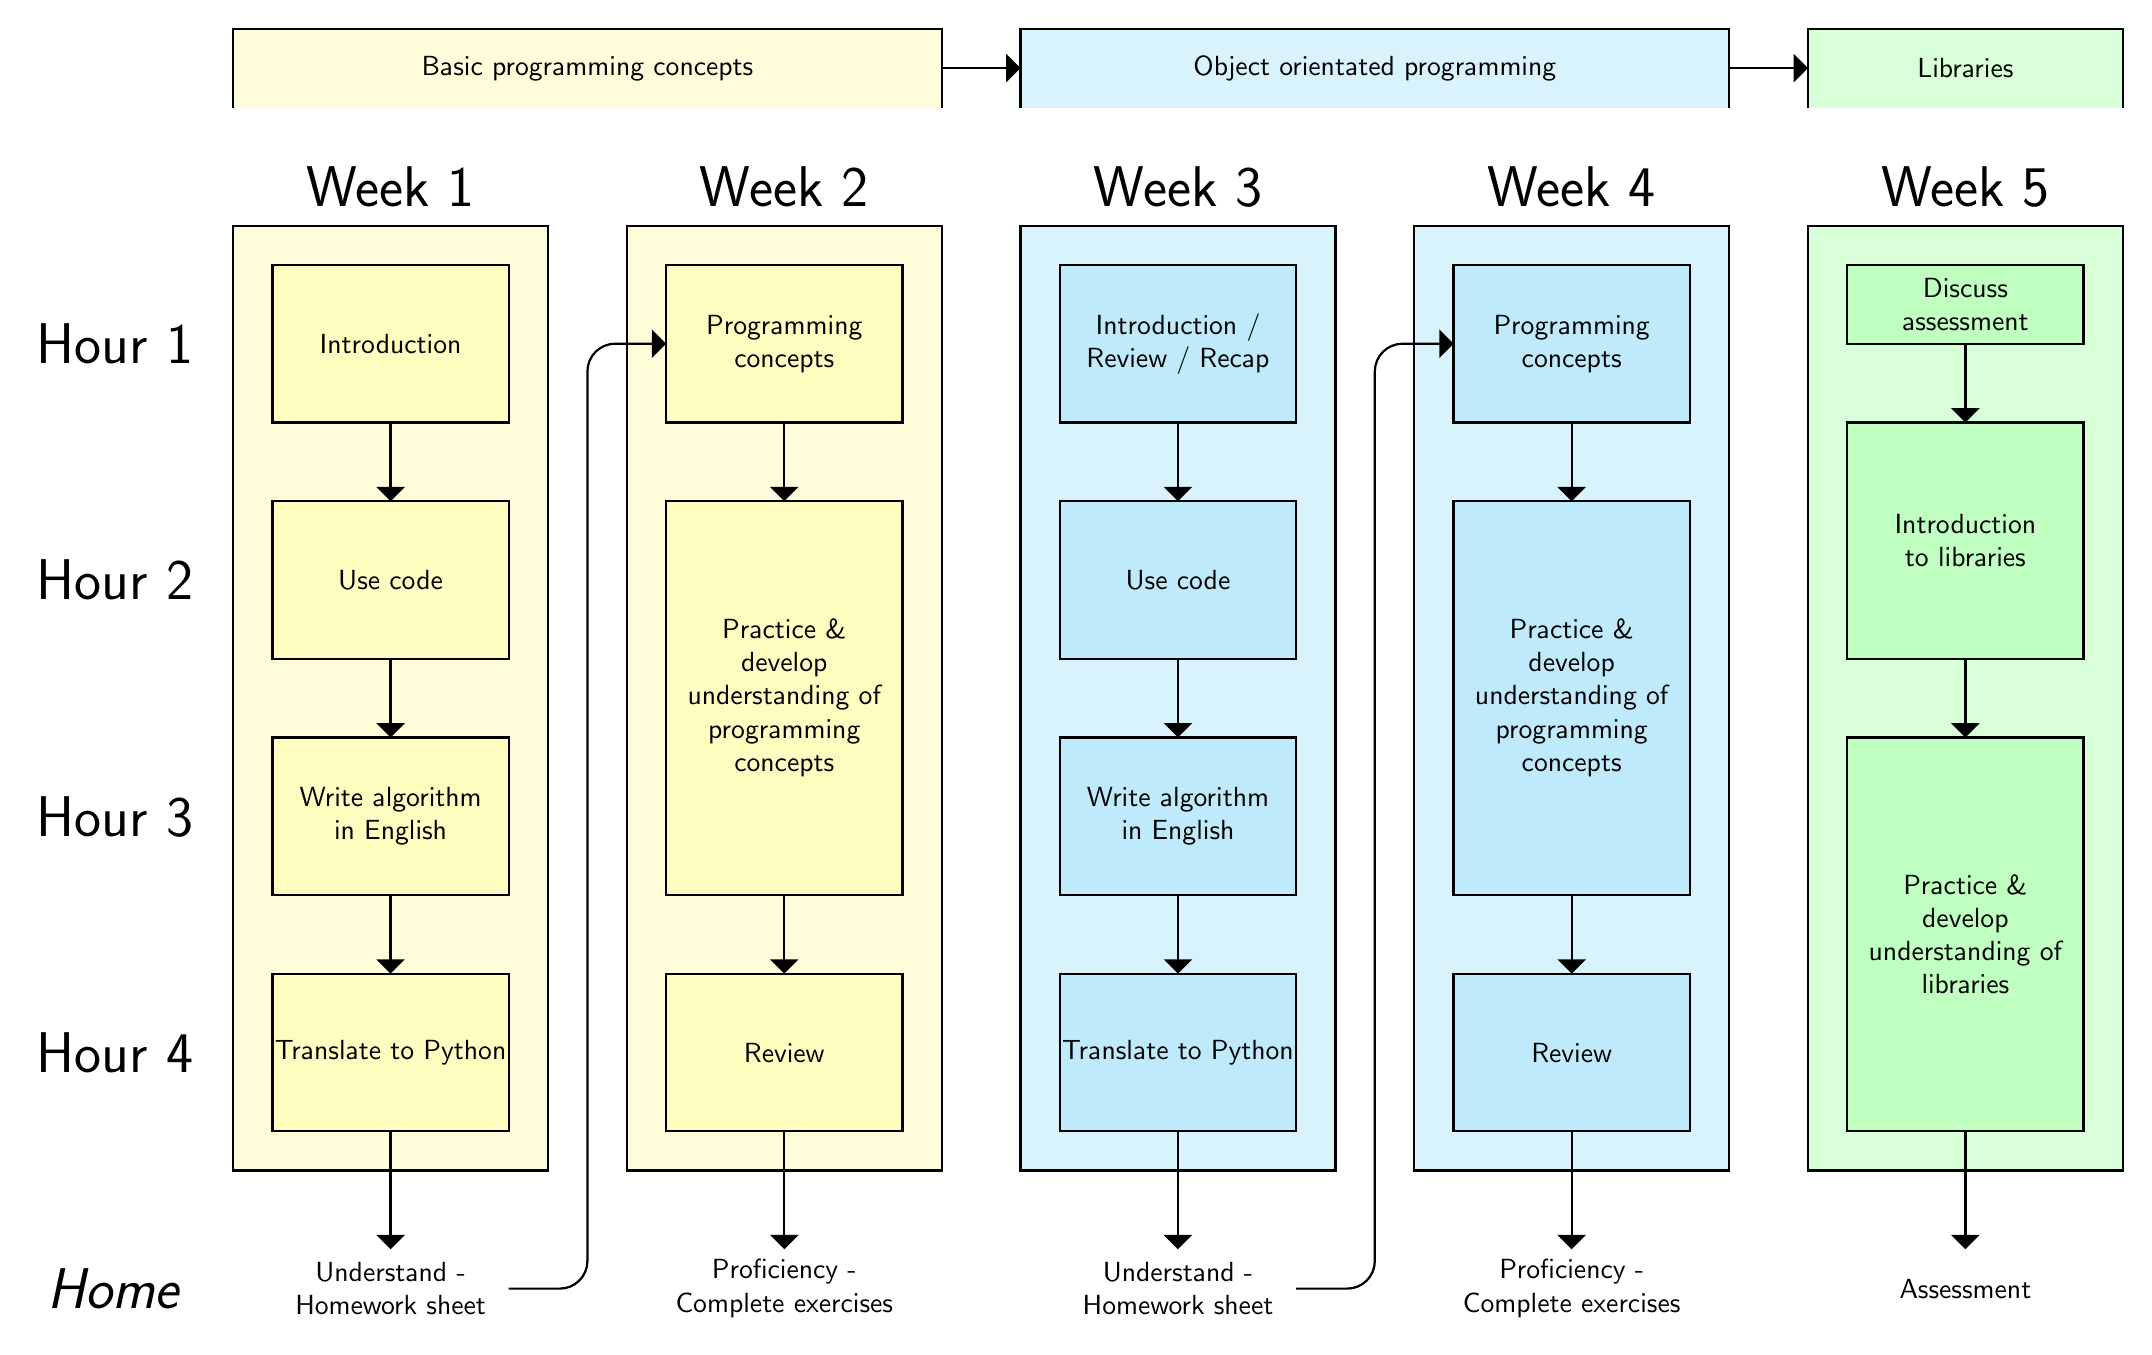
\begin{tikzpicture}

\node at (-2, -2) {\huge \textit{Home}};
\node at (-2, 1) {\huge Hour 4};
\node at (-2, 4) {\huge Hour 3};
\node at (-2, 7) {\huge Hour 2};
\node at (-2, 10) {\huge Hour 1};

\node at (1.5, 12) {\huge Week 1};
\draw[thick, fill=yellow!15] (-0.5, -0.5) rectangle (3.5, 11.5);
\draw[thick, fill=yellow!25] (0, 0) rectangle (3, 2);
\draw[thick, fill=yellow!25] (0, 3) rectangle (3, 5);
\draw[thick, fill=yellow!25] (0, 6) rectangle (3, 8);
\draw[thick, fill=yellow!25] (0, 9) rectangle (3, 11);
\node[align=center] at (1.5, 10) {Introduction};
\node[align=center] at (1.5, 7) {Use code};
\node[align=center] at (1.5, 4) {Write algorithm\\in English};
\node[align=center] at (1.5, 1) {Translate to Python};
\node[align=center] at (1.5, -2) {Understand - \\Homework sheet};

\node at (6.5, 12) {\huge Week 2};
\draw[thick, fill=yellow!15] (4.5, -0.5) rectangle (8.5, 11.5);
\draw[thick, fill=yellow!25] (5, 0) rectangle (8, 2);
\draw[thick, fill=yellow!25] (5, 3) rectangle (8, 8);
\draw[thick, fill=yellow!25] (5, 9) rectangle (8, 11);
\node[align=center] at (6.5, 10) {Programming\\concepts};
\node[align=center] at (6.5, 5.5) {Practice \&\\develop\\understanding of\\programming\\concepts};
\node[align=center] at (6.5, 1) {Review};
\node[align=center] at (6.5, -2) {Proficiency - \\Complete exercises};

\node at (11.5, 12) {\huge Week 3};
\draw[thick, fill=cyan!15] (9.5, -0.5) rectangle (13.5, 11.5);
\draw[thick, fill=cyan!25] (10, 0) rectangle (13, 2);
\draw[thick, fill=cyan!25] (10, 3) rectangle (13, 5);
\draw[thick, fill=cyan!25] (10, 6) rectangle (13, 8);
\draw[thick, fill=cyan!25] (10, 9) rectangle (13, 11);
\node[align=center] at (11.5, 10) {Introduction /\\Review / Recap};
\node[align=center] at (11.5, 7) {Use code};
\node[align=center] at (11.5, 4) {Write algorithm\\in English};
\node[align=center] at (11.5, 1) {Translate to Python};
\node[align=center] at (11.5, -2) {Understand - \\Homework sheet};

\node at (16.5, 12) {\huge Week 4};
\draw[thick, fill=cyan!15] (14.5, -0.5) rectangle (18.5, 11.5);
\draw[thick, fill=cyan!25] (15, 0) rectangle (18, 2);
\draw[thick, fill=cyan!25] (15, 3) rectangle (18, 8);
\draw[thick, fill=cyan!25] (15, 9) rectangle (18, 11);
\node[align=center] at (16.5, 10) {Programming\\concepts};
\node[align=center] at (16.5, 5.5) {Practice \&\\develop\\understanding of\\programming\\concepts};
\node[align=center] at (16.5, 1) {Review};
\node[align=center] at (16.5, -2) {Proficiency - \\Complete exercises};

\node at (21.5, 12) {\huge Week 5};
\draw[thick, fill=green!15] (19.5, -0.5) rectangle (23.5, 11.5);
\draw[thick, fill=green!25] (20, 0) rectangle (23, 5);
\draw[thick, fill=green!25] (20, 6) rectangle (23, 9);
\draw[thick, fill=green!25] (20, 10) rectangle (23, 11);
\node[align=center] at (21.5, 2.5) {Practice \&\\develop\\understanding of\\libraries};
\node[align=center] at (21.5, 7.5) {Introduction\\to libraries};
\node[align=center] at (21.5, 10.5) {Discuss\\assessment};
\node[align=center] at (21.5, -2) {Assessment};

\draw[thick, -triangle 90] (1.5, 9) -- (1.5, 8);
\draw[thick, -triangle 90] (1.5, 6) -- (1.5, 5);
\draw[thick, -triangle 90] (1.5, 3) -- (1.5, 2);
\draw[thick, -triangle 90] (1.5, 0) -- (1.5, -1.5);
\draw[thick, -triangle 90, rounded corners=10pt] (3, -2) -- (4, -2) -- (4, 10) -- (5, 10);

\draw[thick, -triangle 90] (6.5, 9) -- (6.5, 8);
\draw[thick, -triangle 90] (6.5, 3) -- (6.5, 2);
\draw[thick, -triangle 90] (6.5, 0) -- (6.5, -1.5);

\draw[thick, -triangle 90] (11.5, 9) -- (11.5, 8);
\draw[thick, -triangle 90] (11.5, 6) -- (11.5, 5);
\draw[thick, -triangle 90] (11.5, 3) -- (11.5, 2);
\draw[thick, -triangle 90] (11.5, 0) -- (11.5, -1.5);
\draw[thick, -triangle 90, rounded corners=10pt] (13, -2) -- (14, -2) -- (14, 10) -- (15, 10);

\draw[thick, -triangle 90] (16.5, 9) -- (16.5, 8);
\draw[thick, -triangle 90] (16.5, 3) -- (16.5, 2);
\draw[thick, -triangle 90] (16.5, 0) -- (16.5, -1.5);

\draw[thick, -triangle 90] (21.5, 10) -- (21.5, 9);
\draw[thick, -triangle 90] (21.5, 6) -- (21.5, 5);
\draw[thick, -triangle 90] (21.5, 0) -- (21.5, -1.5);

\draw[draw=none, fill=yellow!15] (-0.5, 13) rectangle (8.5, 14);
\draw[thick] (-0.5, 13) -- (-0.5, 14) -- (8.5, 14) -- (8.5, 13);
\node at (4, 13.5) {Basic programming concepts};

\draw[thick, -triangle 90] (8.5, 13.5) -- (9.5, 13.5);

\draw[draw=none, fill=cyan!15] (9.5, 13) rectangle (18.5, 14);
\draw[thick] (9.5, 13) -- (9.5, 14) -- (18.5, 14) -- (18.5, 13);
\node at (14, 13.5) {Object orientated programming};

\draw[thick, -triangle 90] (18.5, 13.5) -- (19.5, 13.5);

\draw[draw=none, fill=green!15] (19.5, 13) rectangle (23.5, 14);
\draw[thick] (19.5, 13) -- (19.5, 14) -- (23.5, 14) -- (23.5, 13);
\node at (21.5, 13.5) {Libraries};

\end{tikzpicture}
\end{document}